\chapter{\label{cha:results}Results}

The aim of this thesis is to gain insight into the behavior and applicability
of heuristics to the task of differential testing of the Kotlin compiler.
To achieve this goal, this chapter seeks to answer the research questions posed in
\Cref{sec:rqs} through empirical evidence and statistical analysis.
We structure the analysis of the results as to mirror the hierarchy
of research questions.
\Cref{sec:resrq1} analyzes the effect of the the most impactful
hyperparameters and the ramifications on the generative heuristics.
\Cref{sec:resrq2} details the performance of the best representative
of each heuristic category.
\Cref{sec:buganalysis} 

\section{\label{sec:resrq1}Influence of Guidance Parameters}

We begin our analysis of hyperparameter influence by considering the effects of
the simplicity bias on the structure, size, and number of files that \kf~ generates
in \Cref{subsec:simpl_bias}, followed by the effects of distance metrics on diversity
heuristics in \Cref{subsec:distance_effect}, and finally, the impact 
of target selection in \Cref{subsec:targets_effect}.

\subsection{\label{subsec:simpl_bias}Effects of Simplicity Bias on Random Sampling}

To study the effects of the simplicity bias, we focus on the size and number of files
generated by \gls{RS}.
We limit the analysis of simplicity bias values to a range between 0.4 and 0.6,
which we empirically evaluated to strike a balance between complexity and size.
Values of this parameter exceeding $0.6$ tend to severely
limit the semantic context in which code is generated,
while values below $0.4$ increase the probability of producing
output whose size and complexity diminish its real-world application.

\begin{figure}[t!]
\centering
\subfigure[Mean size of block generated by \gls{RS} as a function of simplicity bias.]{
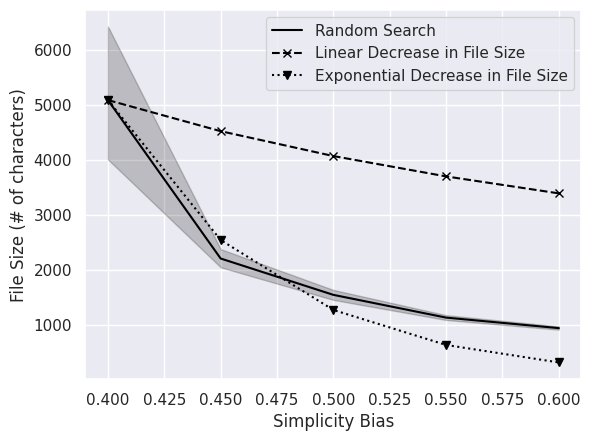
\includegraphics[scale=0.4]{img/rq1-1/lineplot_size.png}
}
\hfill
\subfigure[Number of blocks generated by \gls{RS} per 90 minutes as a function of simplicity bias.]{
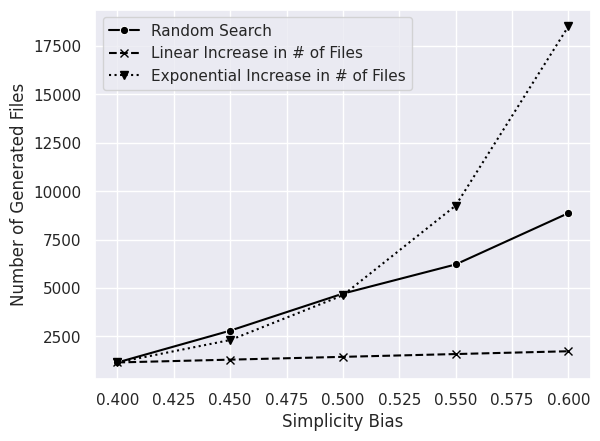
\includegraphics[scale=0.4]{img/rq1-1/lineplot_no_files.png}
}

\caption{Comparison of the number of files generated by \gls{RS} and their size.}
\label{fig:rq1-size-and-number}
\end{figure}

\newacronym{IQR}{IQR}{Inter-Quartile Range}

\Cref{fig:rq1-size-and-number} depicts the relation between (a) the average size of the blocks
generated through random sampling and (b) the number of files the algorithm outputs
in a 90-minute interval.
To help contextualize the rate of change, we introduce additional data
points representing linear (dashed lines) and geometric (dotted lines)
changes in the data, where each previous value is either
halved (for subfigure (a)) or doubled (for subfigure (b)).

For values of the simplicity bias between 0.40 and 0.50, both rates of change
are comparable to their geometric counterparts.
The average size of a file decreases from 5,084 characters for a bias of 0.40
to 2,205 for a bias of 0.45 and 1545 for a bias of 0.50.
The rate of change diminishes for bias values 0.55 and 0.6, with
average sizes of 1,132 and 941 characters, respectively.
Conversely, the number of generated files increases from 
1,157 for the lowest value of bias (0.40) to 8,869 for the highest (0.60).
Values attached to biases between the two extremes follow the same trend,
with 2,799, 4,712, and 6,218 files generated for simplicity biases of
0.45, 0.50, and 0.55, respectively.
Both rates of change significantly outpace their linear equivalents for the entire testes interval.
In isolated cases (first interval for subfigure (a), first two intervals for subfigure (b)),
the rate of change also surpasses its geometric counterpart.

To further understand the variability of random sampling, we consider
the distribution of file sizes for each value of the simplicity bias.
\Cref{fig:rq1-1size-dist} and \Cref{tab:rq1-1size-dist} give the
visual and numerical interpretation of this distribution.
While the mean size of files varies by over 3000 characters between the
extremes of the simplicity bias, the medians only vary by 201.
Further, the the \gls{IQR} more than halves from 2013 for the lowest
simplicity bias, to 834 for the highest.
This suggests that while all tested biases are likely to produce
many files of less than 700 characters, lower simplicity biases
result in many more large outliers than their higher counterparts.
This is in accordance with the depiction of \Cref{fig:rq1-1size-dist},
which highlights that as the simplicity bias increases, its upper quartile
significantly shrinks while the lower quartile remains unchanged.

\begin{minipage}{\textwidth}
  \begin{minipage}[b]{0.49\textwidth}
    \centering
    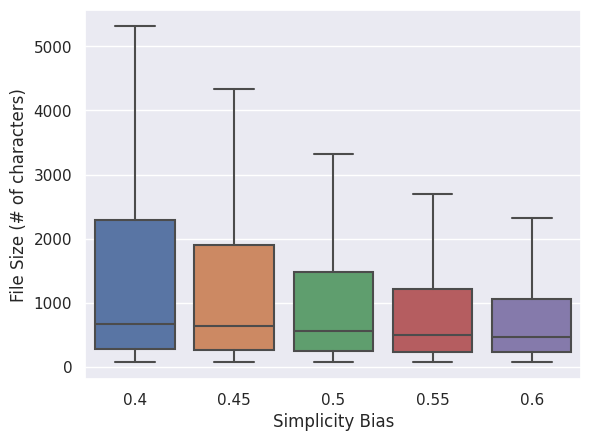
\includegraphics[scale=0.4]{img/rq1-1/boxplot_size.png}
    \captionof{figure}{Distribution of block sizes.}
    \label{fig:rq1-1size-dist}
  \end{minipage}
  \hfill
  \begin{minipage}[b]{0.49\textwidth}
    \centering
\begin{tabular}{c|ccc}
    Bias & Mean & Median & \gls{IQR}\\
    \midrule
    0.40 & 5084 & 669 & 2013\\
    0.45 & 2205 & 644 & 1631\\
    0.50 & 1545 & 555 & 1227\\
    0.55 & 1132 & 499 & 984\\
    0.60 & 941 & 468 & 834
\end{tabular}
\vfill
  \captionof{table}{Block size distribution statistics.}
  \label{tab:rq1-1size-dist}
\end{minipage}
\end{minipage}

\begin{figure}
    \centering
    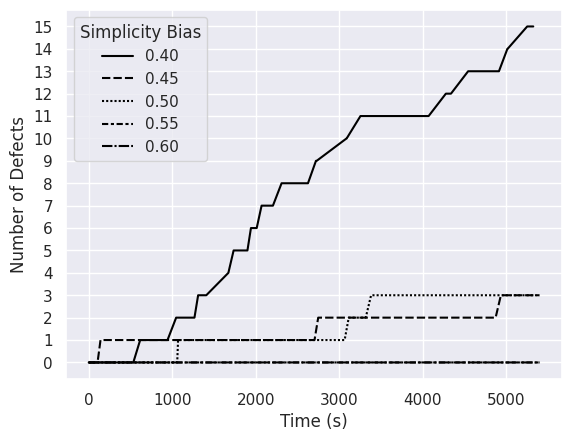
\includegraphics[scale=0.6]{img/rq1-1/convergence-rq-1-1.png}
    \caption{The number of defects uncovered by \gls{RS} over different simplicity bias values.}
    \label{fig:rq1-1convergence}
\end{figure}

\newacronym{OOM}{OOM}{Out-Of-Memory}

Finally, we analyze the relation between the simplicity bias
and the effectiveness of random sampling as a
mechanism for uncovering bugs in the Kotlin compiler.
\Cref{fig:rq1-1convergence} provides a visualization of the number of
defects uncovered through differential testing of the generated files,
for each simplicity bias value tested.
The most important aspect of these results is that \textit{all} defects
uncovered by all 5 versions of \gls{RS} consist of
Type I errors (as described in \Cref{tab:defects}).
These errors all trigger \gls{OOM} errors in the \texttt{K1}
compiler, but not in its newer \texttt{K2} counterpart.

All \gls{OOM} errors encountered in the five experimental runs
exceed 10,000 characters, and their distribution among the
simplicity bias values aligns with the distribution
of file sizes that each value entails.
\gls{RS} with a simplicity bias of 0.40 generates 15 \gls{OOM}-inducing
files, while higher values of 0.45 and 0.50 both produce 3 such instances.
Simplicity bias values exceeding 0.50 do not generate such files,
correlating with their narrower file size distribution.

\begin{center}
    \fbox{
        \begin{minipage}{26em}
            \textbf{Summary RQ1.1}: Lower simplicity bias values cause \gls{RS}
            to generate significantly larger and significantly fewer files,
            given the same computational budget.
            Simplicity biases of 0.50 and lower are likely
            to occasionally generate files of over 
            10,000 characters, which often trigger \gls{OOM} errors in \texttt{K1}, but not in \texttt{K2}.
        \end{minipage}
    }
\end{center}

\subsection{\label{subsec:distance_effect}Effects of Distance Metric on Syntactic Diversity-Driven Search}

We consider the implications of using the $l^2$ and $l^\infty$ norms as distance
measures for \gls{SODGA}.
We additionally take the behavior of \gls{MODGA} into account as a point of comparison,
which does not utilize distance metircs in its optimization.

We begin by analyzing the properties of the files captured in
each snapshot of the algorithms.
\Cref{fig:rq1-2size} provides the visualization of the evolution of the
average generated file size over time.
For both variations of \gls{SODGA}, the mean file size
fluctuates between 1000 and 3500 characters,
which are significantly under the threshold of 10,000 characters
that may trigger common \gls{OOM} errors.
The fluctuations are a consequence of the population-sensitive fitness function:
as the population tends towards larger files, the selection operator
pressures the population towards smaller blocks that inherently 
belong to a farther away region of the search space.
As smaller files take over the population, the trend reverses and larger
files again introduce more diversity.
This trend is apparent for both the $l^2$ and $l^\infty$ norms.
However, the latter introduces larger shifts in the size of blocks because of its
more stringent measure of (dis)similarity.
As a result, the $l^\infty$ variant generates 
both the largest (3500) and smallest (900) average file size population
out of the considered snapshots.

\begin{figure}
    \centering
    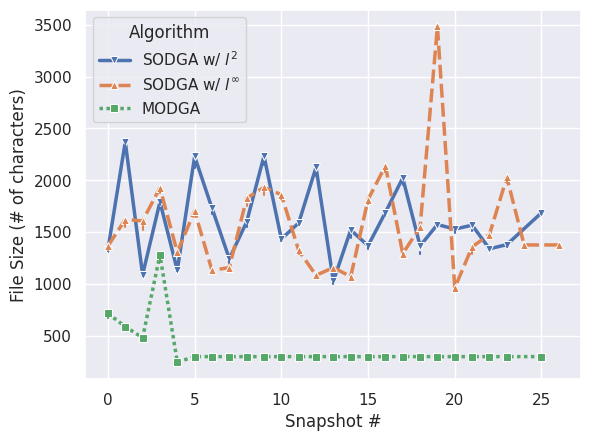
\includegraphics[scale=0.6]{img/rq1-2/rq1-2file-size.png}
    \caption{Mean size of blocks generated by diversity algorithms over time.}
    \label{fig:rq1-2size}
\end{figure}

\begin{minipage}{\textwidth}
\vspace{0.25cm}
  \begin{minipage}[b]{0.49\textwidth}
    \centering
    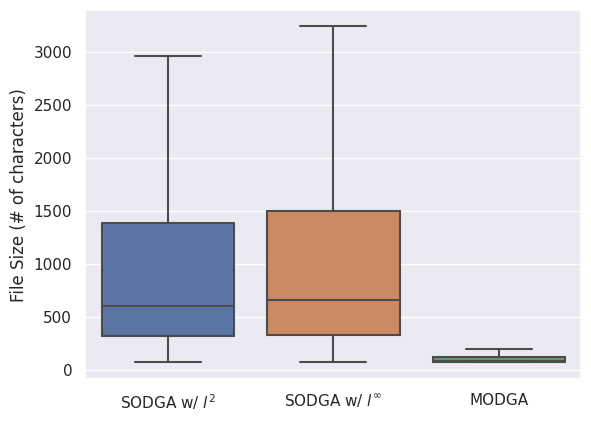
\includegraphics[scale=0.4]{img/rq1-2/rq1-2file-size-dist.png}
    \captionof{figure}{Block size distribution of diversity heuristic variations.}
    \label{fig:rq1-2size-dist}
  \end{minipage}
  \hfill
  \begin{minipage}[b]{0.49\textwidth}
    \centering
\begin{tabular}{c|ccc}
    Variant & Mean & Median & \gls{IQR}\\
    \midrule
    \gls{SODGA}-$l^2$ & 1598 & 599 & 1067\\
    \gls{SODGA}-$l^\infty$ & 1574 & 658 & 1177\\
    \gls{MODGA} & 322 & 83 & 49\\
\end{tabular}
\vfill
  \captionof{table}{Statistics of block size distributions of diversity heuristics.}
  \label{tab:rq1-2size-dist}
\end{minipage}
\vspace{0.25cm}
\end{minipage}

By contrast, the elitist archive of \gls{MODGA} retains files that
are far smaller than the population of its single-objective counterparts.
After initial fluctuations in the first 6 snapshots, the average
size of files in the \gls{MODGA} elitist archive
converges to around 300 characters.
This coincides with the members of the archive itself,
which also converge to a static set of 70 solutions at the sixth snapshot.
Further changes for the remainder of the runtime are minimal by comparison,
as the archive grows by only 3 additional entries.

\Cref{fig:rq1-2size-dist} and \Cref{tab:rq1-2size-dist} provide additional
details regarding the the file size distribution of syntactic diversity heuristics.
The means of the distributions of the two \gls{SODGA} variations
are comparable: the $l^\infty$ variant produces file that are on average only
$1.50\%$ (1574 characters) smaller than the Euclidean norm equivalent (1598 characters).
However, the shape of the distribution differs between the two, with the $l^\infty$ alternative
generating more outliers.
This property reveals itself in the median and \gls{IQR} measures,
which are $9.8\%$ and $10.3\%$ (658 and 1177) larger for 
the $l^\infty$ optimizer than in the Euclidean revision (599 and 1067).
\gls{MODGA} produces files that are both much smaller and less divergent than either
of the single objective options.
This proclivity is attributed to (i) the size component
significantly diminishes the size of the archive and (ii)
the tendency of the archive to retain few ($<$ 10) very large files, which
alone dominate large regions of the search space.

Finally, \Cref{fig:rq1-2convergence} depicts the number of defects uncovered
by each algorithm variation.
Only two defects emerge from differential testing
of the generated files of the three algorithms.
\gls{SODGA} equipped with the $l^\infty$ norm and \gls{MODGA}
each independently uncover one Type III defect that causes
\texttt{K1} to raise an error, while \texttt{K2} successfully
compiles the generated code.
Both instances of the defect emerge as a consequence of the genetic
recombination operator, and could not have been otherwise generated
by \gls{RS}.
We discuss further implications of this defect
and the operators involved in its creation in \Cref{cha:discussion}.

\begin{figure}
    \centering
    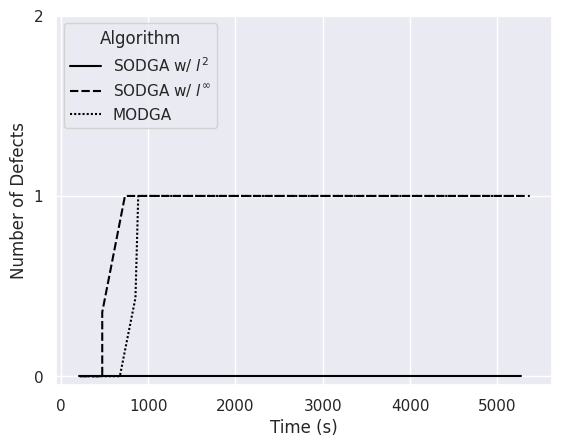
\includegraphics[scale=0.6]{img/rq1-2/rq1-2convergence.png}
    \caption{The number of defects uncovered by \gls{SODGA} and \gls{MODGA}.}
    \label{fig:rq1-2convergence}
\end{figure}

\begin{center}
    \fbox{
        \begin{minipage}{31em}
            \textbf{Summary RQ1.2}: \gls{SODGA} displays comparable
            performance and behavior under both $l^2$ and $l^\infty$ norms,
            with the latter displaying a broader distribution.
            Both variations fluctuate between selecting larger and smaller files,
            based on the algorithm's recent history.
            \gls{MODGA} maintains an archive that stagnates
            after a limited number of iterations, but effectively retains
            smaller files.
            All three algorithms are capable of uncovering defects that \gls{RS} could not.
        \end{minipage}
    }
\end{center}

\subsection{\label{subsec:targets_effect}Effects of Target Set on Semantic Proximity-Driven Search}

We analyze the behavior of \gls{STPGA}, \gls{MOPGA}, and \gls{WSPGA}
under four different target sets, of 50, 100, 200, and 400 targets, respectively.
For each algorithm, we analyze snapshots that consist of either
the closest solution to each target (for \gls{STPGA}),
the set of non-dominated solutions (for \gls{MOPGA}),
or the best suite generated (for \gls{WSPGA}).

We again begin our analysis by considering the size of the files
retained by each algorithm.
The distribution over each snapshot for \gls{STPGA} is given in
\Cref{fig:rq1-3size-dist1} and \Cref{fig:rq1-3size-dist2}.
Means vary by only 14 between the smallest (341 for 400 targets)
and the largest (355 for 200 targets) values.
The file size distribution contains few outliers,
as captured by the \gls{IQR} measurements that do not exceed 260.
While all measurements exceed the size achieved
by \gls{MODGA} (mean 322, \gls{IQR} 49), they are far lower than those
generated by \gls{RS} with an equal simplicity bias (mean 1545, \gls{IQR} 1227).
Since \gls{STPGA} does not contain an explicit size objective like \gls{MODGA},
the only mechanisms to which the retention of smaller files can be attributed to
are either the archival or the embeddings.

\begin{minipage}{\textwidth}
\vspace{0.25cm}
  \begin{minipage}[b]{0.49\textwidth}
    \centering
    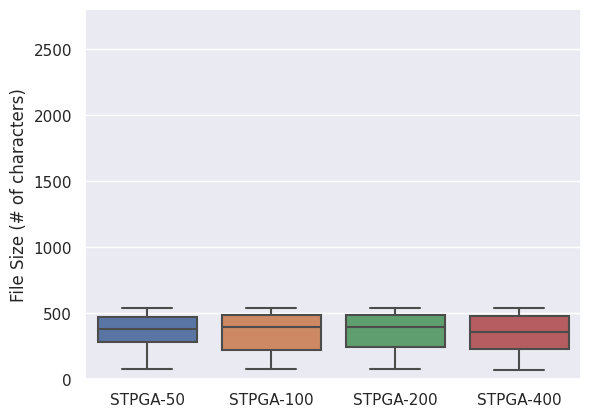
\includegraphics[scale=0.4]{img/rq1-3/rq1-3-size-dist1.png}
    \captionof{figure}{Block size distribution of \gls{STPGA} variations.}
    \label{fig:rq1-3size-dist1}
  \end{minipage}
  \hfill
  \begin{minipage}[b]{0.49\textwidth}
    \centering
\begin{tabular}{c|ccc}
    Variant & Mean & Median & \gls{IQR}\\
    \midrule
    \gls{STPGA}-50 & 353 & 378 & 196\\
    \gls{STPGA}-100 & 350 & 390 & 260\\
    \gls{STPGA}-200 & 355 & 391 & 218\\
    \gls{STPGA}-400 & 341 & 357 & 250\\
\end{tabular}
\vfill
  \captionof{table}{Statistics of block size distributions of \gls{STPGA} variations.}
  \label{tab:rq1-3size-dist1}
\end{minipage}
\vspace{0.25cm}
\end{minipage}

To further understand this phenomenon, we analyze the corresponding behavior
of \gls{MOPGA} and \gls{WSPGA}.
\Cref{fig:rq1-3size-dist2} and \Cref{tab:rq1-3size-dist2} capture the behavior of the former.
While not as drastic, all three measurements of the distribution display significantly lower
values (with means between 986 and 1124, and medians between 344 and 390)
than the \gls{RS} counterpart.
The larger difference between means and medians, together with the
higher \gls{IQR}s highlight the appearance of more outliers in \gls{MOPGA}
than in \gls{STPGA}.
This can, in large part, be attributed to the differences in the implementation
of the archive, which holds far more values for the \gls{MO} variant, and
is thus less stringent on the blocks it retains.

\gls{WSPGA} employs the least constraining retaining mechanism,
simply tracking the test suite with the
best scalarized fitness.
The distribution captured by \Cref{fig:rq1-3size-dist3} and \Cref{tab:rq1-3size-dist3}
reflects this.
\gls{WSPGA} contains, on average, the largest files of any proximity algorithm,
with means more than triple those of \gls{STPGA}.
\gls{WSPGA} also displays the highest variance between its four
versions, with an average difference of 446 characters between
the files pertaining to the \gls{WSPGA}-100 and \gls{WSPGA}-200.
The whole-suite approach also produces the most spread out distribution,
with the highest \gls{IQR} values of all proximity-class methods.
Despite this, all variants of this algorithm retain files that are,
on average, smaller than the \gls{RS} counterpart with the same simplicity bias.

\begin{minipage}{\textwidth}
\vspace{0.25cm}
  \begin{minipage}[b]{0.49\textwidth}
    \centering
    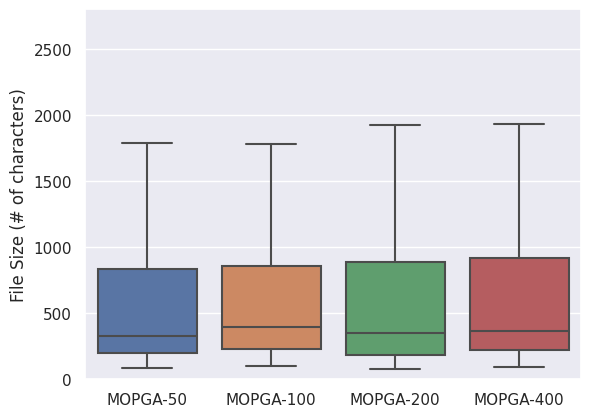
\includegraphics[scale=0.4]{img/rq1-3/rq1-3-size-dist2.png}
    \captionof{figure}{Block size distribution of \gls{MOPGA} variations.}
    \label{fig:rq1-3size-dist2}
  \end{minipage}
  \hfill
  \begin{minipage}[b]{0.49\textwidth}
    \centering
\begin{tabular}{c|ccc}
    Variant & Mean & Median & \gls{IQR}\\
    \midrule
    \gls{MOPGA}-50 & 991 & 378 & 638\\
    \gls{MOPGA}-100 & 986 & 390 & 626\\
    \gls{MOPGA}-200 & 1124 & 344 & 702\\
    \gls{MOPGA}-400 & 988 & 359 & 696\\
\end{tabular}
\vfill
  \captionof{table}{Statistics of block size distributions of \gls{MOPGA} variations.}
  \label{tab:rq1-3size-dist2}
\end{minipage}
\vspace{0.25cm}
\end{minipage}

This phenomenon occurs in all twelve variations, thus suggesting
that the embedding mechanism is the root cause of this bias.
Reasoning about why bias is implanted in the embedding
procedure is difficult, as the \textsc{CodeBERT} \gls{NN} at the core of this process
is hardly interpretable.
However, most files that we include in the target set (or aggregations
emerging as results of operations on the embedding of those files)
are short and contain isolated test cases of specific language features.
This stands out as the most intuitive explanation of the implicit bias
of the algorithm: short generated files embedded by \textsc{CodeBERT} are more likely
to be similar to selected targets, which are also short.
Though this occurrence warrants further investigation, it is outside the scope of this thesis.

\begin{minipage}{\textwidth}
\vspace{0.25cm}
  \begin{minipage}[b]{0.49\textwidth}
    \centering
    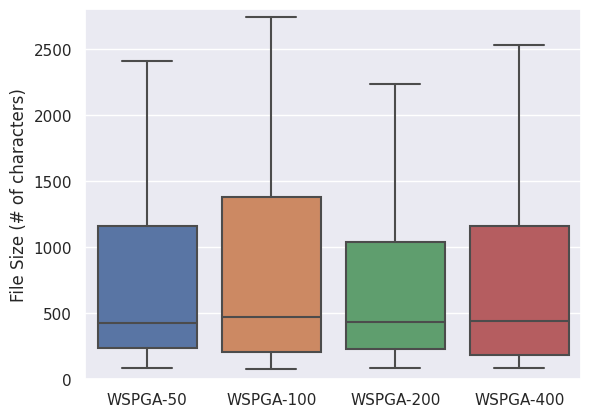
\includegraphics[scale=0.4]{img/rq1-3/rq1-3-size-dist3.png}
    \captionof{figure}{Block size distribution of \gls{WSPGA} variations.}
    \label{fig:rq1-3size-dist3}
  \end{minipage}
  \hfill
  \begin{minipage}[b]{0.49\textwidth}
    \centering
\begin{tabular}{c|ccc}
    Variant & Mean & Median & \gls{IQR}\\
    \midrule
    \gls{WSPGA}-50 & 1053 & 423 & 828\\
    \gls{WSPGA}-100 & 1455 & 468 & 1178\\
    \gls{WSPGA}-200 & 999 & 432 & 816\\
    \gls{WSPGA}-400 & 1109 & 436 & 880\\
\end{tabular}
\vfill
  \captionof{table}{Statistics of block size distributions of \gls{WSPGA} variations.}
  \label{tab:rq1-3size-dist3}
\end{minipage}
\vspace{0.25cm}
\end{minipage}

We additionally consider the behavior over time of the two archive
mechanisms of \gls{STPGA} and \gls{MOPGA}.
This aspect is relevant for understanding the scalability of
the approaches.
Non-dominated archives such as that of \gls{MOPGA}, tend
to scale with the number of solutions in the optimal Pareto set,
which, in general, scales with the number of objectives of the problem \cite{luong2012elitist}.
\Cref{fig:rq1-3archive1} and \Cref{fig:rq1-3archive2} show the behavior of the
archives of \gls{STPGA} and \gls{MOPGA}, respectively.
The former, which only retains the closest block for each target,
behaves as intuitively expected, with variations that have more targets
retaining more files than counterparts with fewer targets.
The number of files retained by the archive of \gls{STPGA} at the end
of the run scales sublinearly with the number of targets,
with \gls{STPGA}-400 only having 5 times more blocks in its archive
than \gls{STPGA}-50, despite having 8 times more targets.
This result implies that scenarios in which one file is the closest approximation
of many targets are common.

\Cref{fig:rq1-3archive2} displays significantly different behavior for \gls{MOPGA}.
Unlike its iterative counterpart, the archive size of \gls{MOPGA} never reaches a stage
where its size converges and fluctuates around a certain value.
Instead, all variations of \gls{MOPGA} grow for the entire duration
of the run, suggesting convergence had not occurred at the end of the experiment.
Additionally, the archive sizes of \gls{MOPGA} variations only scale with the number
of targets in the beginning of the run.
After 6 snapshots (cca. 18 minutes of runtime),
the archives \gls{MOPGA}-50 and \gls{MOPGA}-100 reach the
same size as their higher-target counterparts.
In further snapshots, the variants with the fewest targets
retain the highest number of files.
This occurs as a consequence of the way in which we capture snapshots:
the time-based method we used (intervals of three minutes) does not
take into account the number of generations each algorithm has completed.
\gls{MOPGA} variations with higher numbers of targets incur 
significant overhead as an effect of requiring additional computation with
each iteration, as each archive computation
scales with the number of objectives.
In practice, this means the algorithm progresses at a slower pace
the more objectives it optimizes for, and thus
variants with fewer targets retain more files when runtime is limited.

\begin{minipage}{\textwidth}
\vspace{0.25cm}
  \begin{minipage}[b]{0.49\textwidth}
    \centering
    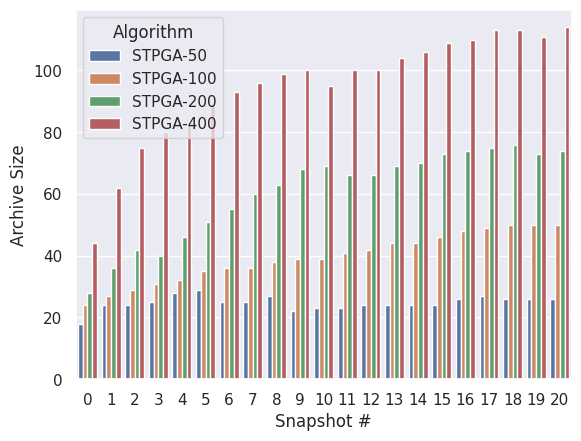
\includegraphics[scale=0.4]{img/rq1-3/rq1-3-archive2.png}
    \captionof{figure}{Evolution of \gls{STPGA} archive size over time.}
    \label{fig:rq1-3archive1}
  \end{minipage}
  \hfill
  \begin{minipage}[b]{0.49\textwidth}
    \centering
    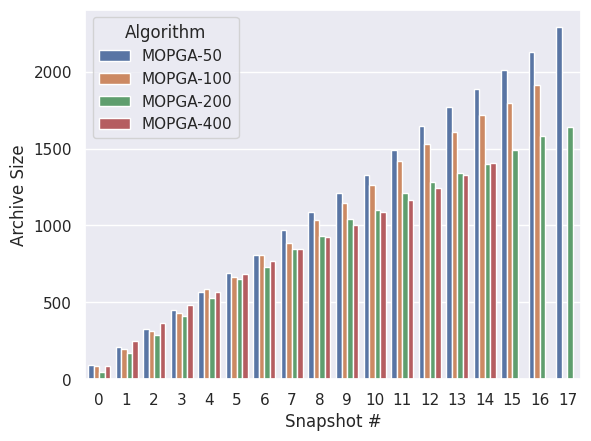
\includegraphics[scale=0.4]{img/rq1-3/rq1-3-archive.png}
    \captionof{figure}{Evolution of \gls{MOPGA} archive size over time.}
    \label{fig:rq1-3archive2}
\end{minipage}
\vspace{0.25cm}
\end{minipage}

Finally, we consider the bug finding capabilities of \gls{STPGA} and \gls{MOPGA},
which are the only two algorithms to uncover defects in our experiments.
\Cref{fig:rq1-3conv1} and \Cref{fig:rq1-3conv2} depict these results, respectively.
While \gls{STPGA} algorithms only uncover one instances of a Type III defect (\texttt{K1} rejects,
\texttt{K2} accepts), \gls{MOPGA} algorithms uncover between 5 and 44 defects each.
These defects include Type II and V \gls{OOM} errors, as well as instances 
of the same Type III defect fond by \gls{STPGA} and diversity-class algorithms.
In addition, \gls{MOPGA} with 400 targets finds the fewest defects (5), 
while \gls{MOPGA}-50 uncovers the most (44).
This coincides with the size of the archives of each algorithm,
with the former having the smallest, and the latter, the largest.
This trend is not entirely consistent with the \gls{MOPGA}-100 and \gls{MOPGA}-200,
with the former finding fewer bugs, despite having the larger archive.

All four algorithms uncover the same \textit{categories} of errors, 
both among themselves, as well as in comparison to diversity algorithms.
This suggests that the number of bugs uncovered by each heuristic is
a consequence of the number of blocks retained in the archive,
rather than a result of the target choice.
Once introduced in the archive, files that cause crashes tend to persist
for the duration of our experiments, thus explaining the consistently increasing
"step size" in the convergence graphs.
The high degree of randomness involved in the generative process, together
with the fact that none of the algorithms had converged at the end of the experiment,
could explain the fact that \gls{MOPGA}-100 and \gls{MOPGA}-200 do not clearly follow this trend.
These results are, however, not conclusive, as we only performed one
run for each variation within this study.
Further analysis based on more empirical data, as well as longer runs that reach convergence,
would improve the understanding of this behavior

\begin{minipage}{\textwidth}
\vspace{0.25cm}
  \begin{minipage}[b]{0.49\textwidth}
    \centering
    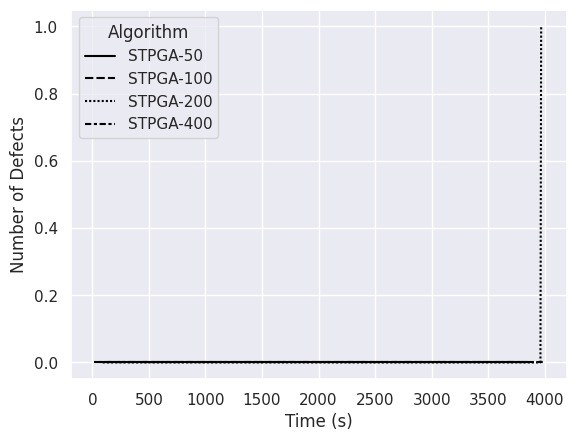
\includegraphics[scale=0.4]{img/rq1-3/rq1-3-conv1.png}
    \captionof{figure}{Evolution of \gls{STPGA} archive size over time.}
    \label{fig:rq1-3conv1}
  \end{minipage}
  \hfill
  \begin{minipage}[b]{0.49\textwidth}
    \centering
    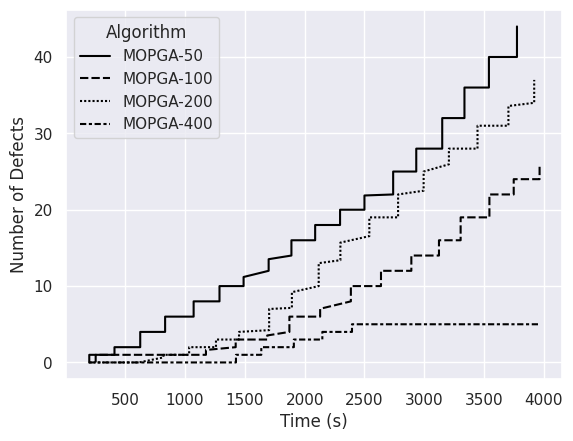
\includegraphics[scale=0.4]{img/rq1-3/rq1-3-conv2.png}
    \captionof{figure}{Evolution of \gls{MOPGA} archive size over time.}
    \label{fig:rq1-3conv2}
\end{minipage}
\vspace{0.25cm}
\end{minipage}

\begin{center}
    \fbox{
        \begin{minipage}{31em}
            \textbf{Summary RQ1.3}: Irrespective of the number of targets,
            all proximity-driven algorithms retain files that are, on average,
            smaller than \gls{RS} with an equivalent simplicity bias, likely
            as a result of biases implanted in the embedding process.
            \gls{STPGA} produces the smallest files, followed by \gls{MOPGA}, and
            \gls{WSPGA}.
            \gls{MOPGA} finds the most defects of any algorithm, which
            is linked to the non-dominated archive retaining files that cause defects
            for long periods of time.
        \end{minipage}
    }
\end{center}

% \begin{figure}[t!]
% \centering
% \subfigure[]{
% 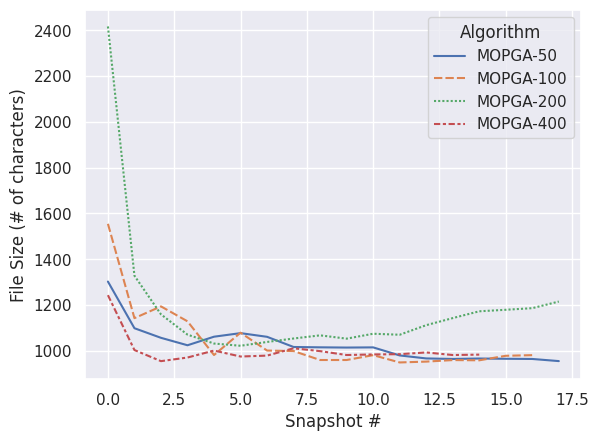
\includegraphics[scale=0.29]{img/rq1-3/rq1-3-size1.png}
% }
% \hfill
% \subfigure[Number of blocks generated by \gls{RS} per 90 minutes as a function of simplicity bias.]{
% 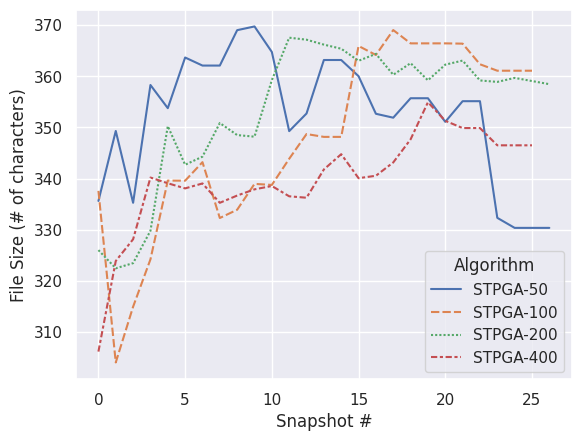
\includegraphics[scale=0.29]{img/rq1-3/rq-1-3-size2.png}
% }
% \hfill
% \subfigure[Number of blocks generated by \gls{RS} per 90 minutes as a function of simplicity bias.]{
% 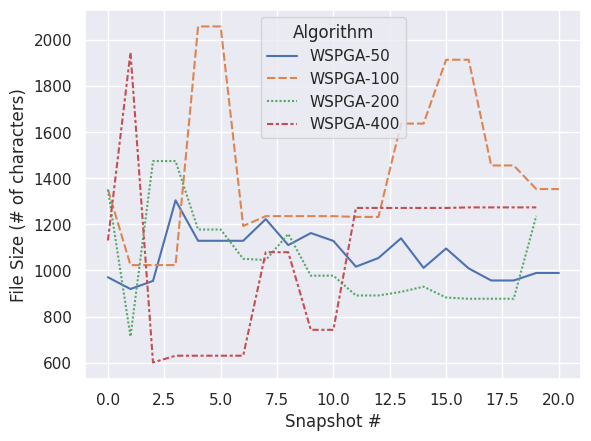
\includegraphics[scale=0.29]{img/rq1-3/rq1-3-size3.png}
% }
% \caption{Comparison of the number of files generated by \gls{RS} and their size.}
% \label{fig:rq1-size-and-number}
% \end{figure}

\section{\label{sec:resrq2}Comparative Heuristic Performance}

To gain additional insight into the comparative performance of the
three classes of heuristics, we compare the
defect uncovering capabilities of one algorithm from each class.
To this end, we performed 10 fuzzing sessions with \gls{RS}, \gls{SODGA}-$l^2$,
and \gls{STPGA}-200, respectively.
We selected \gls{SODGA}-$l^2$ on the basis that it generates
fewer outlier files than its $l^\infty$ counterpart, and does not suffer
from possibly premature convergence, like \gls{MODGA}.
We also selected \gls{STPGA}-200 rather than the \gls{MO}-based counterparts
because the latter's extreme archive growth would make for an unfair
comparison to the other two algorithms, that do not retain such a mechanism.
All algorithms used a simplicity bias of $0.5$.

\begin{minipage}{\textwidth}
\vspace{0.25cm}
  \begin{minipage}[b]{0.3\textwidth}
    \centering
    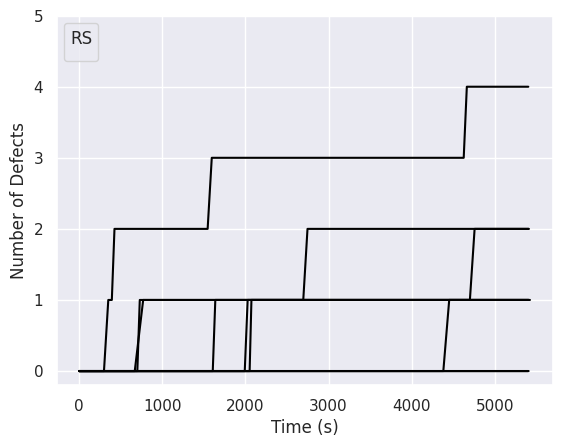
\includegraphics[scale=0.4]{img/rq2/rq2-conv1.png}
    \captionof{figure}{Convergence plot of \gls{RS} defects.}
    \label{fig:rq2conv1}
  \end{minipage}
  \hfill
  \begin{minipage}[b]{0.3\textwidth}
    \centering
    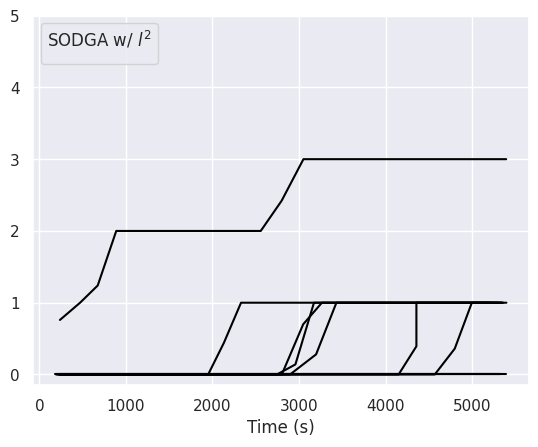
\includegraphics[scale=0.4]{img/rq2/rq2-conv2.png}
    \captionof{figure}{Convergence plot of \gls{SODGA} defects.}
    \label{fig:rq2conv2}
\end{minipage}
  \hfill
  \begin{minipage}[b]{0.3\textwidth}
    \centering
    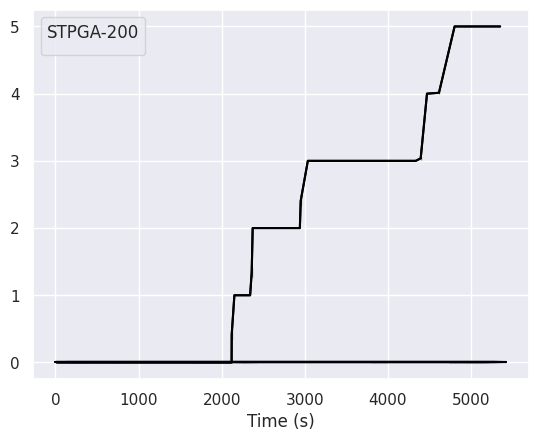
\includegraphics[scale=0.4]{img/rq2/rq2-conv3.png}
    \captionof{figure}{Convergence plot of \gls{STPGA} defects.}
    \label{fig:rq2conv3}
\end{minipage}
\vspace{0.25cm}
\end{minipage}

Figures \Cref{fig:rq2conv1}, \Cref{fig:rq2conv2}, and \Cref{fig:rq2conv3}
show the convergence plots emerging from the three experiments.
\Cref{tab:rq2stats} summarizes the collected metrics and statistical analyses.
In total, \Gls{RS} uncovers more defects (12)
than both \gls{SODGA} (9) and \gls{STPGA} (10).
The statistical analysis of the distribution of the number of bugs
reveals that \gls{RS} is not significantly better at uncovering bugs
than either \gls{SODGA} ($p=0.459$) or \gls{STPGA} ($p=0.570$).
There is also no significant difference in the effectiveness of
\gls{SODGA} and \gls{STPGA} ($p=0.666$).
The \gls{RS} runs reveal one novel Type III defect
(\texttt{K2} does not compile, \texttt{K1} does) not found by any previous experiment,
in addition to several Type II and V errors
(crashes in either just \texttt{K1}, or both \texttt{K1} and \texttt{K2}).
Both the \gls{STPGA} and \gls{SODGA} runs additionally reveal previously
uncovered Type I and Type II defects, and do not generate any novel crashes.
We defer the analysis of individual bugs to \Cref{sec:buganalysis}.

Since all algorithms perform similarly in terms of effectiveness,
we turn to the analysis of efficiency using the \gls{AUC} metric.
The 10 \gls{RS} runs result in the highest mean \gls{AUC} of $0.719$,
which is greater than both \gls{SODGA} ($0.446$) and \gls{STPGA} ($0.385$).
Pairwise statistical analysis shows that no algorithm class is 
statistically better than any other, as per \Cref{tab:rq2stats}.

\begin{table}[h]
    \centering
    \begin{tabular}{c|cc|ccc|ccc}
        &&&\multicolumn{3}{c}{Effectiveness $p$}&\multicolumn{3}{c}{Efficiency $p$}\\
        &\# Defects&Mean \gls{AUC}&\gls{RS} & \gls{SODGA} & \gls{STPGA}&\gls{RS} & \gls{SODGA} & \gls{STPGA}\\
        \midrule
        \gls{RS} &12&0.719 & - & 0.549 & 0.570 & - & 0.322 & 0.400 \\
        \gls{SODGA} &9&0.446&0.549 & - & 0.666 & 0.322 &-& 0.483\\
        \gls{STPGA} &10&0.385& 0.570 & 0.666& - & 0.400 & 0.483 & -\\
    \end{tabular}
    \caption{Summary of effectiveness and efficiency analysis.}
    \label{tab:rq2stats}
\end{table}

To better understand whether the similar behavior in terms of both
effectiveness and efficiency is inherent to our implementation or
a consequence of the relatively limited runtime, we further analyze the empirical behavior
of a longer fuzzer campaign.
We limit this experiment to the same configuration of \gls{SODGA} analyzed
in this section, for three main reasons.
First, the behavior of \gls{SODGA} is transparent, in the sense that it contains no
\gls{BB} components, such as the embeddings of the proximity algorithms, that
could hinder the interpretability of the results.
Second, unlike the proximity-class algorithms and \gls{MODGA}, \gls{SODGA}
evaluates individuals relative to an evolving population.
This volatile fitness function means the algorithm will not converge
upon a stable set of solutions, which is desirable for longer fuzzing campaigns.
Finally, unlike \gls{RS}, \gls{SODGA} leverages both random sampling and genetic operators.

\begin{minipage}{\textwidth}
\vspace{0.25cm}
  \begin{minipage}[b]{0.49\textwidth}
    \centering
    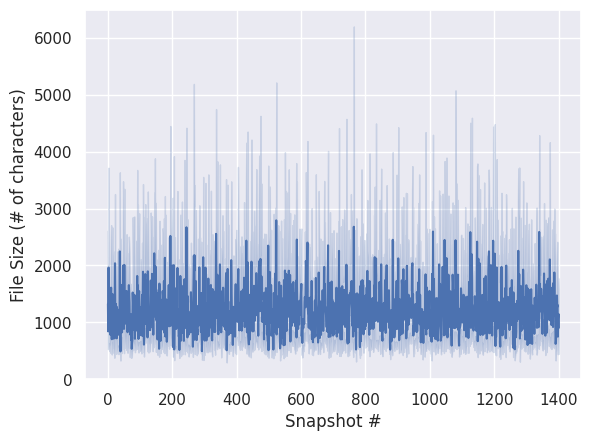
\includegraphics[scale=0.4]{img/rq2/long-exp1.png}
    \captionof{figure}{File size distribution of \gls{SODGA} over 82 hours.}
    \label{fig:rq2long1}
  \end{minipage}
  \hfill
  \begin{minipage}[b]{0.49\textwidth}
    \centering
    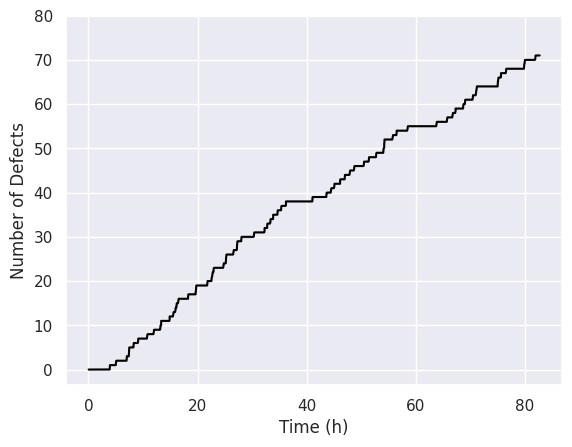
\includegraphics[scale=0.4]{img/rq2/long-exp2.png}
    \captionof{figure}{Convergence plot of \gls{SODGA} defects over 82 hours.}
    \label{fig:rq2long2}
\end{minipage}
\vspace{0.25cm}
\end{minipage}

\Cref{fig:rq2long1} and \Cref{fig:rq2long2} show the results of the long-term experiment.
The fluctuations in size discussed in \Cref{subsec:distance_effect}, that emerge
as a consequence of the population-relative fitness function,
persist for the entire duration of the experiment, as depicted in \Cref{fig:rq2long1}.
In total, the 82 hour fuzzing campaign produced 1401 snapshots and a total of 70,050 files.
Of those files, 70 ($0.099\%$) failed to compile for both \texttt{K1} and \texttt{K2},
as a result of an implementation error in \kf.
The experiment generated 71 files that cause defects, however, no new defects were uncovered.
The 71 files that cause \gls{DT} errors include instances of all previously
uncovered bugs, with the exception of the novel Type III error uncovered by \gls{RS}
and highlighted previously in this section.
We discuss the potential causes underlying this phenomenon in \Cref{cha:discussion}.

\begin{center}
    \fbox{
        \begin{minipage}{31em}
            \textbf{Summary RQ2}: Neither effectiveness, nor efficiency
            are significantly different between
            \gls{RS}, \gls{SODGA}-$l^2$, and \gls{STPGA}-200.
            However, the three algorithms find distinct inidividual categories of defects.
        \end{minipage}
    }
\end{center}

\section{\label{sec:buganalysis}Defect Analysis}

Throughout the experiments carried out in this study, we encountered
several hundred instances of erroneous behavior in the Kotlin compiler.
After individual analysis and consultation with the Kotlin compiler
developer team, we divided these instances into five distinct categories.
This section briefly analyzes these categories, their impact on the Kotlin ecosystem,
and the components of the fuzzer that were responsible for their emergence.

\subsubsection{\texttt{K1} \gls{OOM} Errors}

As our analysis from \Cref{subsec:simpl_bias} revealed, \gls{OOM} errors
occurring only in the \texttt{K1} compiler are common among files that exceed
10,000 characters in length.
The fact that such files do not cause equivalent errors in \texttt{K2}
makes them less important for the scope of this study, as they showcase a measurable
improvement in performance, rather than an issue that requires developer attention.
As a result, we did not report any of these issues to the developer team,
instead focusing on bugs that affect \texttt{K2}.

\subsubsection{\texttt{K2} \gls{OOM} Errors}

We occasionally encountered code that either
(i) triggered \gls{OOM} errors in both \texttt{K1} and \texttt{K2},
or (ii) only triggered \gls{OOM} errors in \texttt{K2}.
Though also large, these files are not as clearly correlated
with size as their \texttt{K1} \gls{OOM} counterparts.
We reported two instances, one for both cases, to the Kotlin developer team.
Compiler developers confirmed both instances for the current release of Kotlin,
and traced the root cause to the compiler's backend \gls{JVM} component.
Both instances were categorized as \textit{perfromance issues}, rather than bugs,
and one of them
\footnote{https://youtrack.jetbrains.com/issue/KT-59190/OutOfMemoryError-Java-heap-space-with-fuzzer-generated-code}
was deemed acceptable. Compiler engineers tracked the root cause of this defect to the quadratic space complexity of a subsystem that performs analysis.
Upon receiving this feedback, we focused our analysis on shorter, more actionable cases.

\begin{figure}[t]
    \centering
    \begin{minted}
    [
    frame=leftline,
    framesep=2mm,
    baselinestretch=1,
    % bgcolor=gray,
    fontsize=\footnotesize,
    linenos
    ]
    {java}
    fun main() {
        fun p () : Char {
            return 'c'
        }
    
        fun p () : Float {
            return 13.0f
        }
    }
    \end{minted}
    \caption{\texttt{K2} false negative conflicting overloads.}
    \label{fig:nested-funcs}
\end{figure}

\subsubsection{\texttt{K2} Nested Functions}

\Cref{fig:nested-funcs} contains a piece of code that triggers a Type I failure.
\texttt{K2} compiles the code without warnings,
while \texttt{K1} fails to do so, and throws a \textit{conflicting overloads} error.
The latter is the intended behavior.
The two \texttt{p} functions cause a resolution conflict that the compiler
is meant to warn of.
After experimentation with this instance, we observed that \texttt{K2} always
resolves a \texttt{p()} function call to the first definition of the function,
irrespective of the return type or the number of re-declarations.
Notably, this problem only occurs when the definitions of \texttt{p()}
are both \textit{nested} inside a higher-scope function.
The Kotlin compiler developers confirmed the existence of this bug
in the current release version, and assigned it medium priority.
The developers additionally fixed a target release date for
a fix in a future minor release of the compiler.

We uncovered several dozen instances of this bug, all generated through
\gls{GA}-based algorithms.
The sampling process that \gls{RS} depends on
contains a check that prevents the generation of functions with
the same name, which is tracked through the share context.
However, this constraint is relaxed during recombination,
allowing for such scenarios to occasionally transpire during crossover.
We further discuss the implications of generative constraints and their
relaxation in \Cref{cha:discussion}.

\subsubsection{\texttt{K2 RuntimeException} }

\Cref{fig:runtime-ex} highlights a Type III error that affects
the \texttt{RuntimeException} class of the Kotlin standard library.
The \texttt{K2} compiler throws an overload resolution ambiguity exception
stemming from the \texttt{RuntimeException(R)} expression in line 3.
\texttt{K1} compiles the code without error, which is the intended behavior.
The Kotlin developers verified the occurrence of this bug in several compiler versions
that were released in 2023, including the most recent one.
The compiler team traced the bug to the resolution and inference components
of the compiler frontend, and assigned a future minor release of Kotlin 1.9
as the target release date for a fix.

Though any permutation of algorithm and configuration described in this study is in
principle capable of generating the code in \Cref{fig:runtime-ex}, it was a
version \gls{RS} not covered in our empirical analysis that first uncovered it.
The 82 hour campaign of \gls{SODGA} subsequently revealed the same defect.
From the perspective of the fuzzer, the piece of code that triggers
the error is a simple fragment generated from an expression node.
Finding such bugs entirely relies on effectively covering the input
of the fuzzer's context, which \gls{RS}-based algorithms
might be more effective at, since they do not incur additional
overhead from other \gls{GA} operators, that operate on higher-levels language structures.

\begin{figure}[h]
    \centering
    \begin{minted}
    [
    frame=leftline,
    framesep=2mm,
    baselinestretch=1,
    % bgcolor=gray,
    fontsize=\footnotesize,
    linenos
    ]
    {java}
    var R: UninitializedPropertyAccessException = UninitializedPropertyAccessException("fooBar")
    R = R ?: UninitializedPropertyAccessException(
        "fooBar".plus(ArithmeticException()), RuntimeException(R))
    \end{minted}
    \caption{\texttt{K2 RuntimeException} overload resolution ambiguity.}
    \label{fig:runtime-ex}
\end{figure}

\subsubsection{\texttt{K2 ConcurrentModificationException}}

Akin to the the \texttt{RuntimeException} scenario, the
code in \Cref{fig:concur-ex} highlights a \texttt{K2}
defect originating from the constructor of
the \texttt{ConcurrentModificationException} class from the Kotlin standard library.
Similar to the previous case, the code surfaced from a fuzzing campaign
of \gls{RS}, in this case from the experiments carried out in \Cref{sec:resrq2}.
Also similar to its peer, this defect was confirmed for the current release of the Kotlin compiler,
and its errors trace back to the same frontend components, called Checkers.
Generating this instance is also feasible for every proposed approach.

\begin{figure}[h]
    \centering
    \begin{minted}
    [
    frame=leftline,
    framesep=2mm,
    baselinestretch=1,
    % bgcolor=gray,
    fontsize=\footnotesize,
    linenos
    ]
    {java}
    var J_: ConcurrentModificationException = ConcurrentModificationException()
    J_ = J_ ?: ConcurrentModificationException(ConcurrentModificationException(J_))
    \end{minted}
    \caption{\texttt{K2 ConcurrentModificationException}  overload resolution ambiguity.}
    \label{fig:concur-ex}
\end{figure}